\documentclass[./RiskyContrib.tex]{subfiles}\providecommand{\econtexRoot}{}
\renewcommand{\econtexRoot}{..}

% Different execution depending on whether compiling main file or as standalone subfile
\onlyinsubfile{\externaldocument{RiskyContrib}} % Get xrefs -- esp to appendix 
%-- from main file; only works properly if main file has already been compiled; 
%order: Compile this file, then main, then this one again
\begin{document}

\hfill{\tiny \texname.tex, \today}

\begin{verbatimwrite}{RiskyContrib.title}  % Write title to .title file
A Two-Asset Savings Model with an Income-Contribution Scheme\\
REMARK
\end{verbatimwrite}

\title{A Two-Asset Savings Model with an Income-Contribution Scheme\\
REMARK}

\author{Mateo Vel\'asquez-Giraldo}

\keywords{Lifecycle, Portfolio Choice, Social Security, Replication}

\maketitle 

\hypertarget{abstract}{}
\begin{abstract}
This paper contains the highlights from the REMARK file in Code>Python folder.
\end{abstract}

% Various resources 
\hypertarget{links}{}
\begin{small}
\parbox{\textwidth}{
\begin{center}
\begin{tabbing}
\texttt{~Archive:~} \= \= \url{http://econ.jhu.edu/people/ccarroll/BufferStockTheory.zip} \kill \\  %
\texttt{~~GitHub:~} \> \> 
\url{http://github.com/econ-ark/REMARK/REMARKS/CGMPortfolio} \\
\texttt{~~~~~~~~~~} \> \> \textit{(In GitHub repo, see \texttt{/Code} for tools for solving and simulating the model)} \\
\end{tabbing}
\end{center}
          
\href{https://mybinder.org/v2/gh/matthew-zahn/CGMPort/develop?filepath=REMARK\%2FCGM_REMARK.ipynb}{CLICK HERE} for an interactive \href{https://en.wikipedia.org/wiki/Project\_Jupyter\#Jupyter_Notebook}{Jupyter Notebook} that uses the \href{https://econ-ark/HARK}{Econ-ARK/HARK} toolkit to produce our figures (warning: it may take several minutes to launch).  Information about citing the toolkit can be found at \href{https://econ-ark.org/acknowledging/}{Acknowleding Econ-ARK}.
} % end parbox{\textwidth}
\end{small}

\begin{authorsinfo}
\name{Contact: \href{mailto:mvelasq2@jhu.edu}{\texttt{mvelasq2@jhu.edu}}, \href{mailto:matthew.zahn@jhu.edu}{\texttt{matthew.zahn@jhu.edu}}, Department of Economics, 590 Wyman Hall, Johns Hopkins University, Baltimore, MD 21218, \url{https://t.co/uaflostQyF?amp=1}, \url{http://matthewvzahn.com}.}
\end{authorsinfo}

\thanks{All numerical results herein were produced using the \href{https://econ-ark/HARK}{Econ-ARK/HARK} toolkit; for further reference options see \href{https://econ-ark.org/acknowledging/}{Acknowleding Econ-ARK}.  Thanks to Chris Carroll and Sylvain Catherine for comments and guidance.}

\titlepagefinish

\newtheorem{defn}{Definition}
\newtheorem{theorem}{Theorem}

\hypertarget{Introduction}{}
\section{Introduction}

This paper develops a two-asset consumption-savings model and serves as
the documentation of an open-source implementation of its
solution and simulation methods in the \href{https://econ-ark.org/toolkit}{HARK}
toolkit \citep{carroll2018HARK}. The model represents an agent who can
save using two different assets---one risky and the other risk-free---to insure
against fluctuations in his income, but faces frictions to transferring funds between
assets. The flexibility of its implementation and its inclusion in the HARK
toolkit allows users to adapt the model to realistic life-cycle calibrations, and
also to embedded it in heterogeneous-agents macroeconomic models.

\textbf{Macro applications}
The last decade of research in macroeconomics has experienced and increased
interest in how households allocate their savings to assets with different
risk exposures and liquidity. Heterogeneous asset allocations have been shown
to be determinant to the effects of fiscal and monetary policy
\citep{Kaplan2014ecta,Luetticke2021aej_macro}.

\textbf{Micro applications}

\hypertarget{The model}{}
\section{The model}

I now discuss the main components of the model informally, and leave its full
recursive mathematical representation for Section \ref{sec:recursive}.

\subsubsection{Time, mortality, and utility}

Time advances in discrete steps that I will index with $t$. The model can
be used in both infinite and finite-horizon versions.

Agents face an exogenous risk of death $\delta_t$ each period, which becomes certain at the 
maximum age of the finite-horizon version. There are no intentional bequests; agents
will consume all of their resources if they reach the last period, but they can leave
accidental bequests upon premature death.

In each period, agents derive utility from consumption only. Their utility function
follows a constant relative risk aversion specification. Formally, for a level of 
consumption $C$, the agent derives instant utility
\begin{equation}
	u(C) = \frac{C^{1-\rho}}{1- \rho}.
\end{equation}

\subsubsection{Income process}

Agents supply labor inelastically. Their labor earnings $Y_{i,t}$ are the product of a
permanent component $P_{i,t}$ and a transitory stochastic component $\theta_{i,t}$ as
in \cite{Carroll1997qje},  where $i$ indexes different agents. Formally,
\begin{equation*}
\begin{split}
\ln Y_{i,t} &= \ln P_{i,t} + \ln \theta_{i,t} \\
\ln P_{i,t} &= \ln P_{i,t-1} + \ln \Gamma_{i,t} + \ln \psi_{i,t}
\end{split}
\end{equation*}
where $\Gamma_{i,t}$ is a deterministic growth factor that can capture
life-cycle patterns in earnings, and
$\ln \psi_{i,t}\sim \mathcal{N}(-\sigma^2_{\psi,t}/2, \sigma_{\psi,t})$
is a multiplicative shock to permanent income\footnote{The mean of the shock is set so that $E[\psi_{i,t}] = 1$.}.

The transitory component $\theta_{i,t}$ is a mixture that models unemployment and
other temporal fluctuations in income as
\begin{equation*}
\ln\theta_{i,t} = \begin{cases}
\ln \mathcal{U}, & \text{With probability } \mho\\
\ln \tilde{\theta}_{i,t}\sim\mathcal{N}(-\sigma^2_{\theta,t}/2, \sigma_{\theta,t}), & \text{With probability } 1-\mho,
\end{cases}
\end{equation*}
with $\mho$ representing the probability of unemployment and $\mathcal{U}$ the replacement
factor of unemployment benefits.

This specification of the income process is parsimonious and flexible enough to accommodate
life-cycle patterns in income growth and volatility, transitory unemployment and exogenous
retirement. Introduced by \cite{Carroll1997qje}, this income specification is common in studies
of life-cycle wealth accumulation and portfolio choice; see e.g.,
\cite{Cagetti2003jbes,Cocco2005rfs,Fagereng2017jof}. The specification has
also been used in studies of income volatility, which have yielded calibrations of its stochastic
shocks' distributions \citep[see e.g.,][]{Carroll1992bpea,Carroll1997jme,Sabelhaus2010jme}

\subsubsection{Financial assets and frictions}\label{sec:fin_frictions}

Agents smooth their consumption by saving and have two assets
available for this purpose. The first is a risk-free liquid account with 
constant per-period return factor $R$. The second has a stochastic return
factor $\tilde{R}$ that is log-normally distributed and independent across
time. Various interpretations such as stocks, a retirement fund, or entrepreneurial
capital could be given to the risky asset. Importantly, consumption must be paid for
using funds from the risk-free account. The levels of risk-free and risky assets
owned by the agent will both be state variables, denoted with $M_{i,t}$ and $N_{i,t}$
respectively.

Portfolio rebalancing takes place by moving funds between the risk-free
and risky accounts. These flows are one of the agents' control variables
and are denoted as $D_{i,t}$, with $D_{i,t}>0$ representing a movement of
funds from the risk-free to the risky account. Withdrawals from the risky
account are subject to a constant-rate tax $\tau$ which can represent, for
instance, capital-gains realization taxes or early retirement-fund withdrawal
penalties. In sum, denoting post-rebalancing asset levels with $\tilde{\cdot}$,
\begin{equation*}
\begin{split}
\tilde{M}_{i,t} &= M_{i,t} - D_{i,t}(1 - 1_{[D_{i,t}\leq0]}\tau)\\
\tilde{N}_{i,t} &= N_{i,t} + D_{i,t}.
\end{split}
\end{equation*}

At any given period, an agent might not be able to rebalance his portfolio.
This ability is governed by an exogenous stochastic shock that is realized
at the start of the period
\begin{equation*}
\Adj_t \sim \text{Bernoulli}(p_t),
\end{equation*}
with $\Adj_t=1$ meaning that the agent can rebalance and $\NAdj_t=1$ ($\Adj_t = 0$)
forcing him to set $D_{i,t} = 0$. This friction is a parsimonious way to capture
the fact that portfolio rebalancing is costly and households do it sporadically.
Recent studies have advocated for \citep{Giglio2021aer} and used
\citep{Luetticke2021aej_macro} this kind of rebalancing friction.

To partially evade the possibility of being unable to rebalance their accounts, agents
can use an income deduction scheme. By default, labor income ($Y_{i,t}$) is deposited to
the risk-free liquid account at the start of every period. However, agents can pre-commit
to have a fraction  $\Contr_t\in[0,1]$ of their income diverted to their risky account instead.
This fraction can be tweaked by the agent whenever $\Adj_t = 1$; otherwise it stays at its
previous value, $\Contr_{t+1} = \Contr_t$.

\subsubsection{Timing}

\begin{figure}
\begin{center}
\resizebox{\linewidth}{!}{
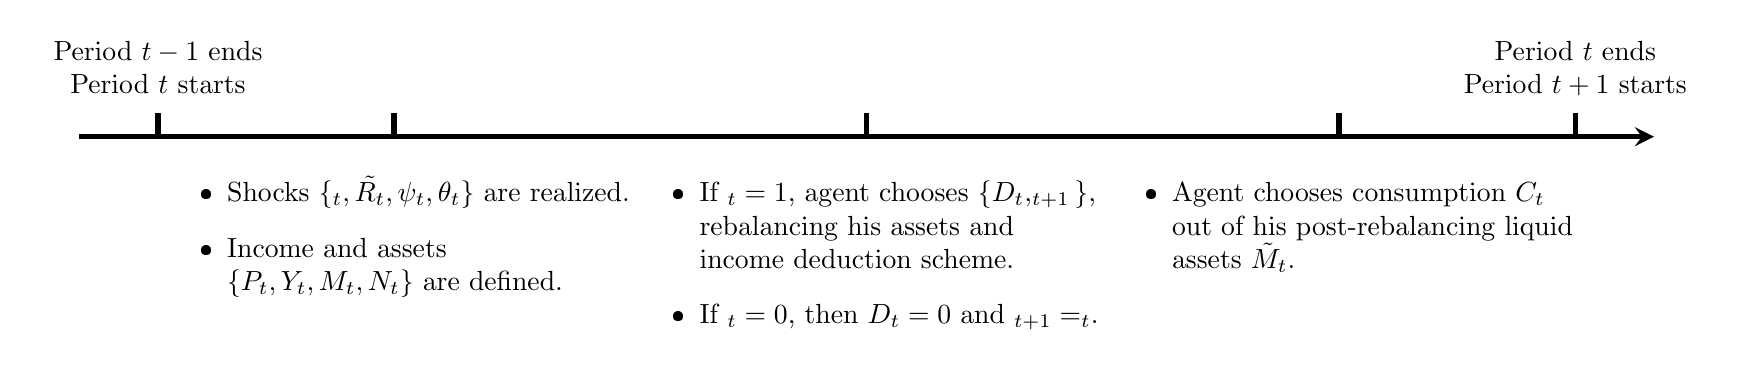
\begin{tikzpicture}
\usetikzlibrary{calc}

% draw arrow
\coordinate (start) at (-3,0);
\coordinate (end) at (17,0);

\draw [line width=2pt, -stealth] (start) -- (end);

% Priod ticks
\coordinate (period_s) at ($(start) + (1,0)$);
\coordinate (period_st) at ($(period_s) + (0,0.3)$);
\coordinate (period_e) at ($(end) - (1,0)$);
\coordinate (period_et) at ($(period_e) + (0,0.3)$);

\draw [line width=2pt] (period_s) -- (period_st);
\node [anchor=south] at (period_st.north) {\begin{tabular}{c}
Period $t-1$ ends \\ Period $t$ starts
\end{tabular}};

\draw [line width=2pt] (period_e) -- (period_et);
\node [anchor=south] at (period_et.north) {\begin{tabular}{c}
Period $t$ ends \\ Period $t+1$ starts
\end{tabular}};

% You can use `foreach` to improve the following codes
\coordinate (s0) at (1,0);
\coordinate (t0) at ($(s0)+(0,0.3)$);
\coordinate (s1) at (7,0);
\coordinate (t1) at ($(s1)+(0,0.3)$);
\coordinate (s2) at (13,0);
\coordinate (t2) at ($(s2)+(0,0.3)$);

% draw ticks
\draw [line width=2pt] (s0) -- (t0);
\node [anchor=south] at (t0.north) {};

\draw [line width=2pt] (t1) -- (s1);
\node [anchor=south] at (t1.north) {};

\draw [line width=2pt] (t2) -- (s2);
\node [anchor=south] at (t2.north) {};

% add texts
\node [anchor=north, align=left, text width=6cm] at (s0.south) {
\begin{itemize}
\item Shocks $\{\Adj_t,\tilde{R_t}, \psi_t, \theta_t\}$ are realized.
\item Income and assets $\{P_t, Y_t, M_t, N_t\}$ are defined.
\end{itemize}
};

\node [anchor=north, align=left, text width=6cm] at (s1.south) {
\begin{itemize}
\item If $\Adj_t=1$, agent chooses $\{D_t,\Contr_{t+1}\}$, rebalancing
his assets and income deduction scheme.
\item If $\Adj_t = 0$, then $D_t =0$ and $\Contr_{t+1} = \Contr_t$.
\end{itemize}
};

\node [anchor=north, align=left, text width=6cm] at (s2.south) {
\begin{itemize}
\item Agent chooses consumption $C_t$ out of his post-rebalancing
liquid assets $\tilde{M}_t$.
\end{itemize}
};
\end{tikzpicture}
}

\caption{Summary of the Model's Timing}\label{fig:Timing_diagram}
\end{center}
\end{figure}

Figure \ref{fig:Timing_diagram} summarizes the timing of stochastic shocks and
optimizing decisions that occur within a period of the life cycle model.

\hypertarget{Recursive}{}
\section{Recursive representation of the model}\label{sec:recursive}

Individual subscripts are dropped for simplicity. The value function for
an agent who is not allowed to rebalance his portfolio at time $t$ is
\begin{equation*}
    \begin{split}
V^{\NAdj}_{t}(M_t, N_t, P_t, \Contr_t) = \max_{C_t} u(C_t) 
+ p_{t+1} &\beta\delta_{t+1} E_t \left[  V^{\Adj}_{t+1}\left( M_{t+1}, N_{t+1}, 
P_{t+1} \right)\right] +\\
\left(1-p_{t+1}\right) &\beta\delta_{t+1} E_t\left[V^{\NAdj}_{t+1}\left(M_{t+1}, 
N_{t+1}, P_{t+1}, \Contr_{t+1}\right) \right]\\
\text{Subject to:} \quad &\\
0\leq& C_t \leq M_t \\
A_t =& M_t - C_t \\
M_{t+1} =& R A_t + (1-\Contr_{t+1}) Y_{t+1}\\
N_{t+1} =& \tilde{R}_{t+1}N_t + \Contr_{t+1}Y_{t+1}\\
P_{t+1} =& \Gamma_{t+1} \psi_{t+1} P_{t}\\
Y_{t+1} =& \theta_{t+1} P_{t+1}\\
\Contr_{t+1} =& \Contr_t
\end{split}
\end{equation*}
and that of agent who is allowed to rebalance is
\begin{equation*}
    \begin{split}
V^{\Adj}_{t}(M_t, N_t, P_t) = \max_{C_t,D_t,\Contr_{t+1}} 
u(C_t) + p_{t+1} &\beta\delta_{t+1} E_t \left[  V^{\Adj}_{t+1}\left( M_{t+1}, 
N_{t+1}, P_{t+1} \right)\right] +\\
\left(1-p_{t+1}\right) &\beta\delta_{t+1} E_t\left[V^{\NAdj}_{t+1}\left(M_{t+1}, 
N_{t+1}, P_{t+1}, \Contr_{t+1}\right) \right]\\
\text{Subject to:} \quad &\\
\quad -N_t \leq D_t \leq M_t, \quad \Contr_{t+1} \in& [0,1], \quad 0 \leq C_t \leq \tilde{M}_t\\
\hfill\\
\tilde{M}_t =& M_t - D_t\left(1-1_{[D_t\leq0]}\tau\right)\\
\tilde{N}_t =& N_t + D_t\\
A_t =& \tilde{M}_t - C_t \\
M_{t+1} =& R A_t + (1-\Contr_{t+1}) Y_{t+1}\\
N_{t+1} =& \tilde{R}_{t+1} \tilde{N}_t + \Contr_{t+1}Y_{t+1}\\
P_{t+1} =& \Gamma_{t+1}\psi_{t+1} P_{t}\\
Y_{t+1} =& \theta_{t+1} P_{t+1}
\end{split}
\end{equation*}

The problem can be normalized by permanent income, following
\cite{Carroll2020solvingmicrodsops}. Using lower case variables to
denote their upper-case counterparts normalized by permanent income ($x_t \equiv X_t/P_t$)
and defining $\tilde{\Gamma}_t = \Gamma_{t}\psi_{t}$, we can write
normalized problems
\begin{equation}\label{eq:bellman_NAdj_norm}
\begin{split}
v^{\NAdj}_{t}(m_t, n_t, \Contr_t) = \max_{c_t} u(c_t) 
+ p_{t+1} &\beta\delta_{t+1} E_t \left[ \tilde{\Gamma}_{t+1}^{1-\rho} v^{\Adj}_{t+1}\left( m_{t+1}, n_{t+1}\right)\right] +\\
\left(1-p_{t+1}\right) &\beta\delta_{t+1} E_t\left[\tilde{\Gamma}_{t+1}^{1-\rho} v^{\NAdj}_{t+1}\left(m_{t+1}, 
n_{t+1}, \Contr_{t+1}\right) \right]\\
\text{Subject to:} \quad &\\
0\leq& c_t \leq m_t \\
a_t =& m_t - c_t \\
m_{t+1} =& \frac{R}{\tilde{\Gamma}_{t+1}} a_t + (1-\Contr_{t+1}) \theta_{t+1}\\
n_{t+1} =& \frac{\tilde{R}_{t+1}}{\tilde{\Gamma}_{t+1}}n_t + \Contr_{t+1}\theta_{t+1}\\
\Contr_{t+1} =& \Contr_t
\end{split}
\end{equation}
and
\begin{equation*}
\begin{split}
v^{\Adj}_{t}(m_t, n_t) = \max_{c_t,d_t,\Contr_{t+1}} 
u(c_t) + p_{t+1} &\beta\delta_{t+1} E_t \left[ \tilde{\Gamma}_{t+1}^{1-\rho}  v^{\Adj}_{t+1}\left( m_{t+1}, 
n_{t+1} \right)\right] +\\
\left(1-p_{t+1}\right) &\beta\delta_{t+1} E_t\left[\tilde{\Gamma}_{t+1}^{1-\rho} v^{\NAdj}_{t+1}\left(m_{t+1}, 
n_{t+1}, \Contr_{t+1}\right) \right]\\
\text{Subject to:} \quad &\\
-n_t \leq d_t \leq m_t, \quad \Contr_{t+1} \in& [0,1], \quad 0 \leq c_t \leq \tilde{m}_t\\
\hfill\\
\tilde{m}_{t} =& m_t - d_t\left(1-1_{[d_t\leq0]}\tau\right)\\
\tilde{n}_{t} =& n_t + d_t\\
a_t =& \tilde{m}_t - c_t \\
m_{t+1} =& \frac{R}{\tilde{\Gamma}_{t+1}} a_t + (1-\Contr_{t+1})\theta_{t+1}\\
n_{t+1} =& \frac{\tilde{R}_{t+1}}{\tilde{\Gamma}_{t+1}}\tilde{n}_{t} + \Contr_{t+1}\theta_{t+1}
\end{split}
\end{equation*}
It can be shown that
\begin{equation*}
V_{t}^{\Adj}(M_t,N_t,P_t) = P_t^{1-\rho} v_{t}^{\Adj}(m_t,n_t), \quad
V_{t}^{\NAdj}(M_t,N_t,P_t,\Contr_t) = P_t^{1-\rho} v_{t}^{\NAdj}(m_t,n_t,\Contr_t),
\end{equation*}
and that the policy functions of both problems are related through
\begin{equation*}
\begin{split}
C_t^{\NAdj}(M_t,N_t,P_t,\Contr_t) = P_t c_t^{\NAdj}(m_t,n_t,\Contr_t),& \quad C_t^{\Adj}(M_t,N_t,P_t) = P_t c_t^{\Adj}(m_t,n_t),\\
D_t(M_t,N_t,P_t) = P_t d_t(m_t,n_t),& \quad \Contr_{t+1}(M_t,N_t) = \Contr_{t+1}(m_t,n_t).
\end{split}
\end{equation*}
Therefore, the model's implementation solves the problem in normalized form, and re-scales
the relevant states and choices using permanent income when simulating.

\subsection{Partition into stages}

An additional insight that facilitates solving the model is that the three decisions
that an agent might take in a period (rebalancing his assets, choosing his income
deduction fraction and consuming) can be seen as happening sequentially. This is
convenient because:
\begin{itemize}
\item The sub-problems are easier to solve than the multi-choice full problem.
\item Since the non-adjusting agent only chooses his consumption and we must
solve his problem for every combination of $(m_t, n_t, \zeta_t=\zeta_{t+1})$, we can re-utilize
his solution by expressing the adjusting agent's  problem as
\begin{equation*}
v_t^{\Adj}(m_t,n_t) = \max_{\tilde{m}_t, \tilde{n}_t, \Contr_{t+1}} v_t^{\NAdj}(\tilde{m}_t, \tilde{n}_t, \Contr_{t+1}).
\end{equation*}
This insight is similar to the ``nested'' reformulation suggested by \cite{Druedahl2020compecon}.
\end{itemize}

To start re-expressing the problem, I take the order of the ageent's decisions to be:
rebalance assets, define income contribution share and finally consume. I denote the stages
at which these decisions are taken with $\Reb$, $\Sha$, and $\Cns$ respectively. I will use
$v^{\Reb}(\cdot)$, $v^{\Sha}(\cdot)$ and $v^{\Cns}(\cdot)$ to represent
\emph{stage value functions}.

I now present each stage in detail, working backwards in time.

\subsubsection{Consumption stage, $\Cns$}

An agent who takes his assets and income contribution share as given is one who
can not adjust them and can only choose his consumption. This corresponds to the
problem of the non-adjusting agent (Equation \ref{eq:bellman_NAdj_norm}). The
important facts to realize at this stage are that
\begin{equation*}
v_t^{\Adj}(m_t, n_t) = v_t^{\Reb}(m_t, n_t), \quad v_t^{\NAdj}(m_t, n_t, \Contr_t) = v_t^{\Cns}(m_t, n_t, \Contr_t),
\end{equation*}
with the first fact being true because we have assumed that asset rebalancing
is the first decision that an adjusting agent takes, and he assumes that his
subsequent decisions will be optimal. Therefore, the consumption stage problem is
\begin{equation*}
\begin{split}
v^{\Cns}_{t}(\tilde{m}_t, \tilde{n}_t, \Contr_{t+1}) = \max_{c_t} u(c_t) 
+ p_{t+1} &\beta\delta_{t+1} E_t \left[ \tilde{\Gamma}_{t+1}^{1-\rho} v^{\Reb}_{t+1}\left( m_{t+1}, n_{t+1}\right)\right] +\\
\left(1-p_{t+1}\right) &\beta\delta_{t+1} E_t\left[\tilde{\Gamma}_{t+1}^{1-\rho} v^{\Cns}_{t+1}\left(m_{t+1}, 
n_{t+1}, \Contr_{t+1}\right) \right]\\
\text{Subject to:} \quad &\\
0\leq& c_t \leq \tilde{m}_t \\
a_t =& \tilde{m}_t - c_t \\
m_{t+1} =& \frac{R}{\tilde{\Gamma}_{t+1}} a_t + (1-\Contr_{t+1}) \theta_{t+1}\\
n_{t+1} =& \frac{\tilde{R}_{t+1}}{\tilde{\Gamma}_{t+1}}\tilde{n}_t + \Contr_{t+1}\theta_{t+1}
\end{split}
\end{equation*}

\subsubsection{Income contribution share stage, $\Sha$}

An agent with the option to set his income contribution share will do so
taking his asset allocation as given and assuming that he will optimally
pick his consumption in the next stage. His problem is
\begin{equation*}
v_t^{\Sha}(\tilde{m}_t,\tilde{n}_t) = \max_{\zeta_{t+1}\in[0,1]} v^{\Cns}_{t}(\tilde{m}_t, \tilde{n}_t, \Contr_{t+1})
\end{equation*}

\subsubsection{Rebalancing stage, $\Reb$}

The first decision that an agent takes, if allowed, is how to reallocate his
assets. At this stage, his value function is
\begin{equation*}
\begin{split}
v^{\Reb}_{t}(m_t, n_t) =& \max_{d_t} v_t^{\Sha}(\tilde{m}_t, \tilde{n}_t)\\
\text{Subject to:} \quad &\\
-n_t \leq& d_t \leq m_t\\
\tilde{m}_{t} =& m_t - d_t\left(1-1_{[d_t\leq0]}\tau\right)\\
\tilde{n}_{t} =& n_t + d_t\\
\end{split}
\end{equation*}

\hypertarget{Solutions}{}
\section{Solutions}

\subsection{Infinite-horizon}

\hypertarget{inf_dFunc}{}
\begin{figure}[tbp]
\centerline{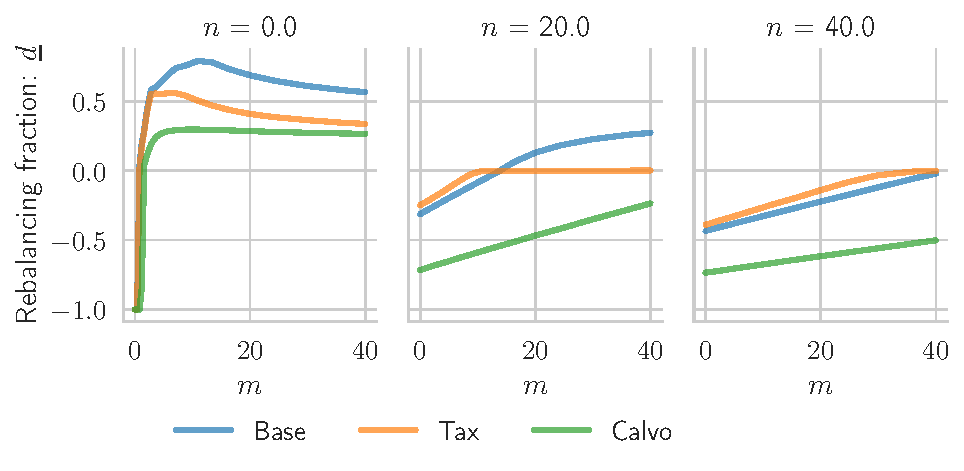
\includegraphics[]{\FigDir/inf_dFunc}}
\caption{Optimal rebalancing fraction $\dFrac$ in the infinite horizon model.}
\label{fig:inf_dFunc}
\end{figure}
\hypertarget{inf_ShareFunc}{}
\begin{figure}[tbp]
\centerline{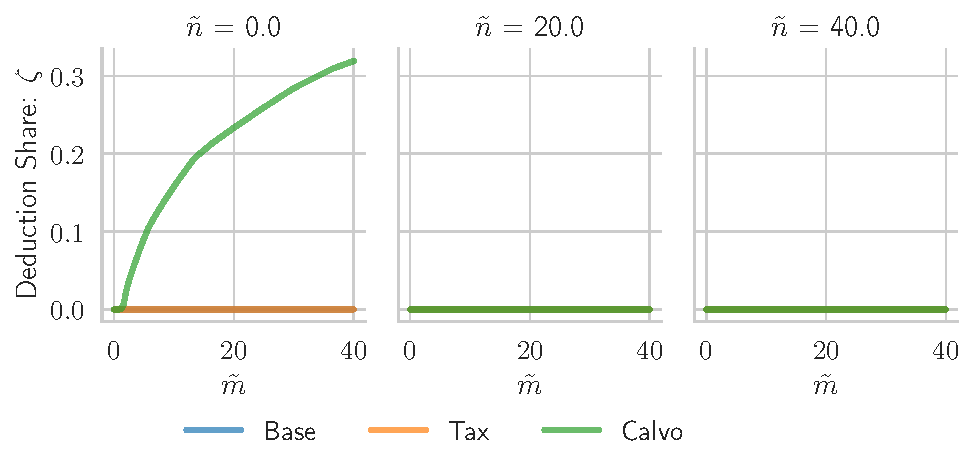
\includegraphics[]{\FigDir/inf_ShareFunc}}
\caption{Optimal income contribution share $\Contr$ in the infinite horizon model.}
\label{fig:inf_ShareFunc}
\end{figure}
\hypertarget{inf_cFunc}{}
\begin{figure}[tbp]
\centerline{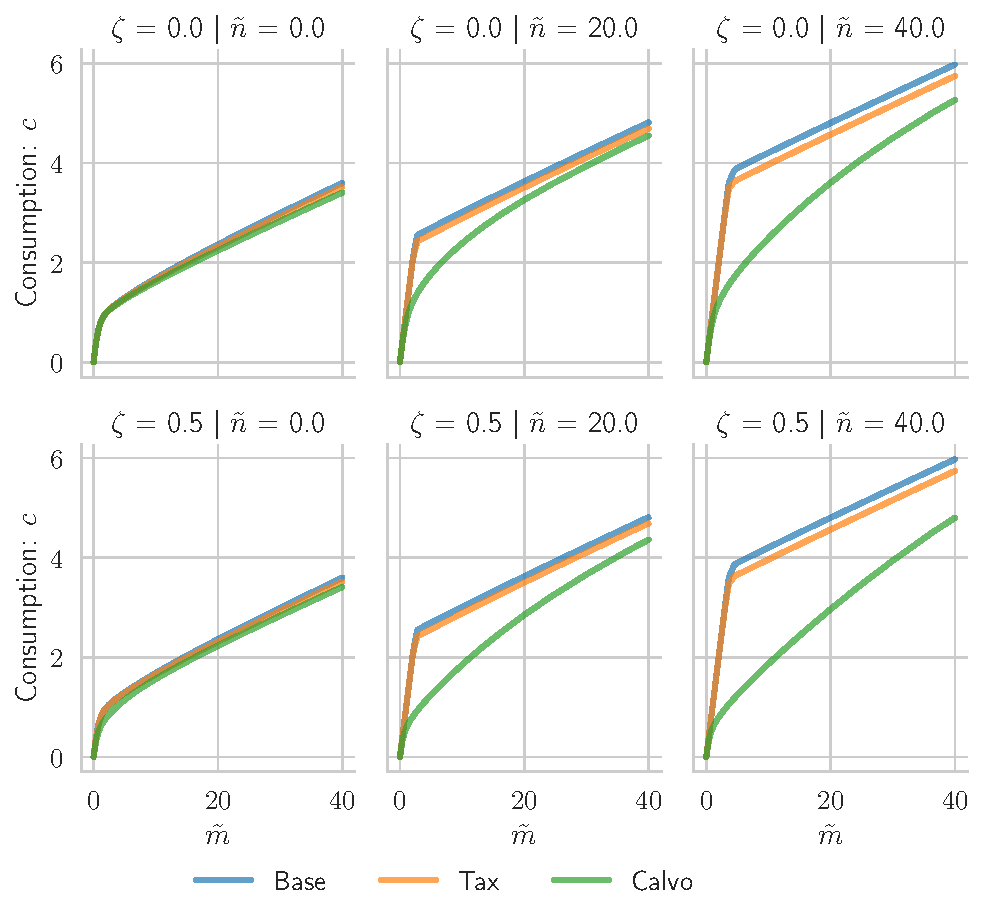
\includegraphics[]{\FigDir/inf_cFunc}}
\caption{Convergence of the Consumption Rules}
\label{fig:inf_cFunc}
\end{figure}

\subsection{Life-Cycle finite horizon}

\hypertarget{LC_age_profiles}{}
\begin{figure}[tbp]
\centerline{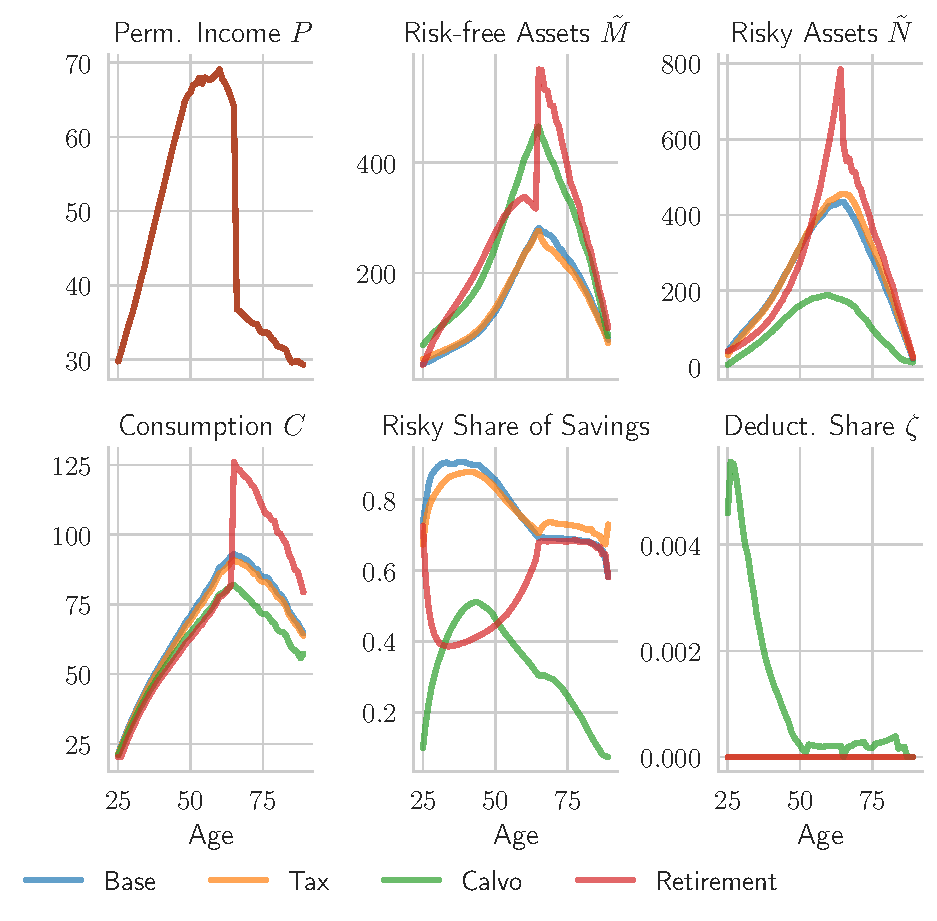
\includegraphics[]{\FigDir/LC_age_profiles}}
\caption{Age profiles of variables of interest in life-cycle calibrations}
\label{fig:LC_age_profiles}
\end{figure}

\hypertarget{Conclusion}{}
\section{Conclusion}

\hypertarget{Puzzles-and-Questions}{}
\section{Puzzles and Questions}\label{sec:Puzzles}

\hypertarget{Robustness Analyses}{}
\section{Robustness Analyses}

\clearpage\vfill\eject

\onlyinsubfile{\bibliography{\econtexRoot/RiskyContrib-Add}}

\end{document}
